\chapter{Introduction}
\label{sec:introduction}
\section{Motivation}
\label{sec:motivation}
A need for synthetic data distributions is on the rise and the trend doesn't seem to slow down. 
The last years held great advantages in the field of generative models, especially in the domain of image generation.
Big institutions like OpenAI, StabilityAI or others provided the necessary velocity that drove mayor improvements. Starting out with rather
poor results the models were capable of learning basic contexts of images but the overall quality was bad. In the following years a new architecture
emerged \cite{ho_denoising_2020} \cite{nichol_improved_2021} and soon outperformed the former best performing models \cite{dhariwal_diffusion_2021}. 
Those rapid improvements led to a high velocity research environment regarding this topic. Commercial and open-source applications like DALLE or Stable Diffiusion emerged.
As seen in fig. \ref{fig:sd images} open source models like Stable Diffusion empower people to generate their own images locally on their home computer.
These applications mostly relied on Denoising Diffusion Probabilistic Models (DDPM). After achieving such great results in the domain of image generation, the decision was made to apply those models to another domain of data - specifically, time series data. Reworking the DDPM architecture so it can handle time series samples is the main task. This might lead
to a new way of synthesizing time series data. DDPM consist only of one model that is easy to understand and training is a simple process, which give them a practical advantage.
In comparison to one other prominent model type like Generative Adversarial Networks \cite{Goodfellow_2017}, DDPM don't rely on a second model which renders the training significantly less complex.
\begin{figure*}
    \centering
    \begin{subfigure}{0.5\textwidth}
        \centering
        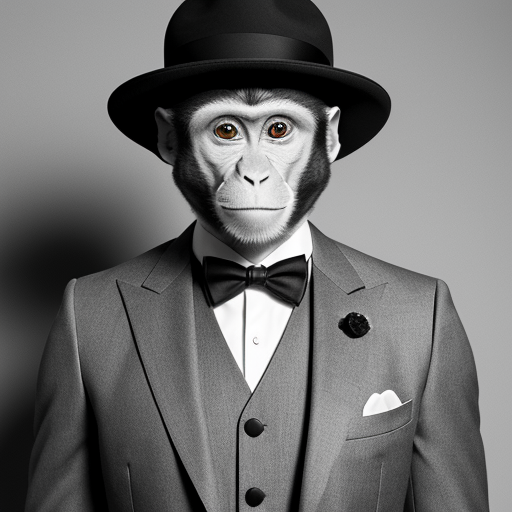
\includegraphics[width=0.5\linewidth]{images/sd1.png}
        \caption[Monkey with tuxedo and hat]%
        {{\small Monkey with tuxedo and hat}}    
        \label{fig:sd1}
    \end{subfigure}%
    \begin{subfigure}{0.5\textwidth}  
        \centering 
        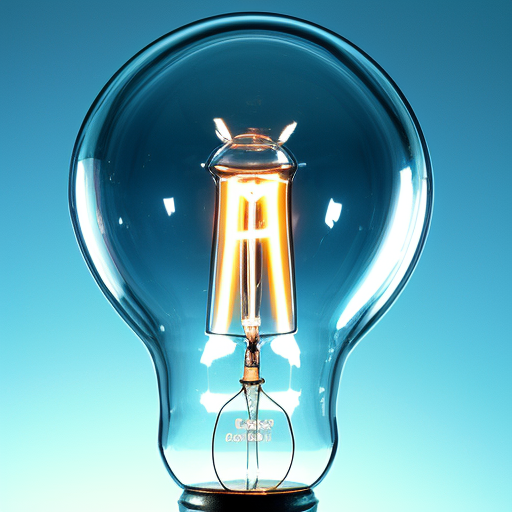
\includegraphics[width=0.5\linewidth]{images/sd2.png}
        \caption[Light bulb]%
        {{\small Light bulb}}    
        \label{fig:sd2}
    \end{subfigure}\\
    \begin{subfigure}{0.5\linewidth}   
        \centering 
        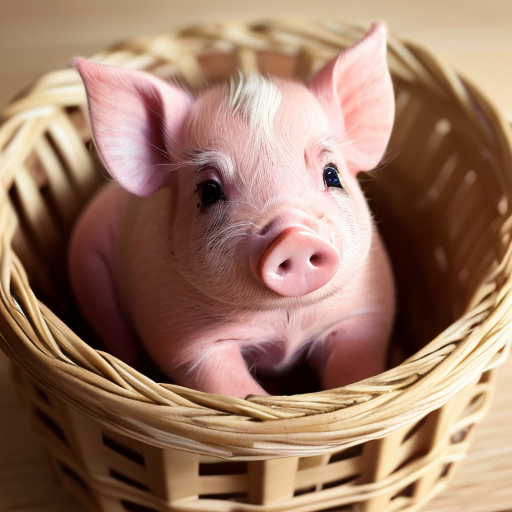
\includegraphics[width=0.5\linewidth]{images/sd3.png}
        \caption[Pig in a basket]%
        {{\small Pig in a basket}}    
        \label{fig:sd3}
    \end{subfigure}%
    \begin{subfigure}{0.5\linewidth}   
        \centering 
        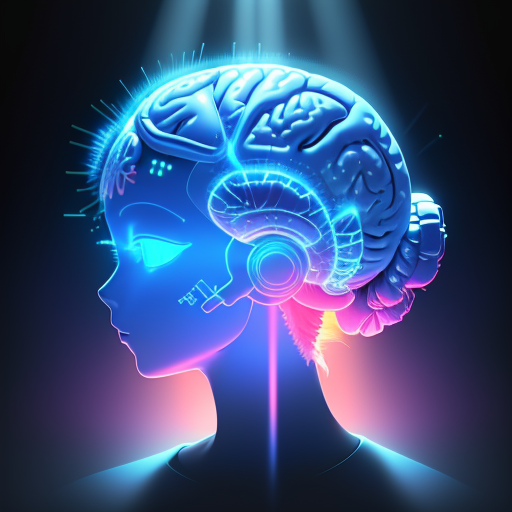
\includegraphics[width=0.5\linewidth]{images/sd4.png}
        \caption[Artistic depiction of an AI]%
        {{\small Artistic depiction of an AI}}    
        \label{fig:sd4}
    \end{subfigure}%
    \caption[ Locally generated images using Stable Diffusion 1.5 ]
    {\small Locally generated images using Stable Diffusion 1.5.} 
    \label{fig:sd images}
\end{figure*}

\section{Contribution}
\label{sec:contribution}

The contribution of this thesis is to investigate whether DDPM are considerable models for the task of 
time series synthesis. Representing the information context of a certain time series distribution can have a supportive
role for different anonymization tasks, forecasting task and data pipelines. For this purpose, the DDPM architecture was reworked to align with the requirements of working with time series data. Following a set of statistical means is defined to evaluate the generated samples.
As another layer of evaluation an applicative test is introduced. This test consists of using our trained models in continual learning scenario, so this thesis also shines light on the question if 
a trained DDPM can perform in a Continual Learning environment that is based on time series data.

\section{Content Structure}
\label{sec:contentstructure}

This section gives an overview of the contents of each chapter in this thesis.

\textbf{Chapter \ref{sec:introduction} Introduction}

A basic summarization of the contents that are presented in this thesis.

\textbf{Chapter \ref{sec:foundations} Foundations}

An overview and comprehensive explanation of all foundations that are necessary to understand the contents of this thesis.

\textbf{Chapter \ref{sec:stateoftheart} State of the art}

A look into the scientific landscape surrounding the questions that are investigated in this thesis.
Naming different approaches that where considered by others to answer the same or similar questions.

\textbf{Chapter \ref{sec:approach} Approach}

A description of the implemented methods and models. Showing a sketch of the framework that was build.

\textbf{Chapter \ref{sec:datasets} Datasets}

An overview of all datasets that were used for the machine learning tasks. Also details about the structure, size and content of each dataset.

\textbf{Chapter \ref{sec:experiments} Experiments}

A definition of specific experimental environments that are used to guaranty a coherent evaluation of the results gathered during 
the investigations.

\textbf{Chapter \ref{sec:results} Results}

An evaluation and discussion of the results that were found during the experiments.

\textbf{Chapter \ref{sec:application} Applications}

A description of different sectors or fields of research this work can be practically used in. 

\textbf{Chapter \ref{sec:conclusion} Conclusion}

A final conclusion that summarizes all results and answers that where found during the thesis work.



